%%%%%%%%%%%%%%%%%%%%%%%%%%%%%%%%%%%%%%%%%
% Beamer Presentation
% LaTeX Template
% Version 1.0 (10/11/12)
%
% This template has been downloaded from:
% http://www.LaTeXTemplates.com
%
% License:
% CC BY-NC-SA 3.0 (http://creativecommons.org/licenses/by-nc-sa/3.0/)
%
%%%%%%%%%%%%%%%%%%%%%%%%%%%%%%%%%%%%%%%%%

%----------------------------------------------------------------------------------------
%	PACKAGES AND THEMES
%----------------------------------------------------------------------------------------

\documentclass{beamer}

\mode<presentation> {

% The Beamer class comes with a number of default slide themes
% which change the colors and layouts of slides. Below this is a list
% of all the themes, uncomment each in turn to see what they look like.

%\usetheme{default}
%\usetheme{AnnArbor}
%\usetheme{Antibes}
%\usetheme{Bergen}
%\usetheme{Berkeley}
%\usetheme{Berlin}
%\usetheme{Boadilla}
%\usetheme{CambridgeUS}
%\usetheme{Copenhagen}
%\usetheme{Darmstadt}
%\usetheme{Dresden}
%\usetheme{Frankfurt}
%\usetheme{Goettingen}
%\usetheme{Hannover}
%\usetheme{Ilmenau}
%\usetheme{JuanLesPins}
%\usetheme{Luebeck}
\usetheme{Madrid}
%\usetheme{Malmoe}
%\usetheme{Marburg}
%\usetheme{Montpellier}
%\usetheme{PaloAlto}
%\usetheme{Pittsburgh}
%\usetheme{Rochester}
%\usetheme{Singapore}
%\usetheme{Szeged}
%\usetheme{Warsaw}

% As well as themes, the Beamer class has a number of color themes
% for any slide theme. Uncomment each of these in turn to see how it
% changes the colors of your current slide theme.

%\usecolortheme{albatross}
%\usecolortheme{beaver}
%\usecolortheme{beetle}
%\usecolortheme{crane}
%\usecolortheme{dolphin}
%\usecolortheme{dove}
%\usecolortheme{fly}
%\usecolortheme{lily}
%\usecolortheme{orchid}
%\usecolortheme{rose}
%\usecolortheme{seagull}
%\usecolortheme{seahorse}
%\usecolortheme{whale}
%\usecolortheme{wolverine}

%\setbeamertemplate{footline} % To remove the footer line in all slides uncomment this line
%\setbeamertemplate{footline}[page number] % To replace the footer line in all slides with a simple slide count uncomment this line

%\setbeamertemplate{navigation symbols}{} % To remove the navigation symbols from the bottom of all slides uncomment this line
}

\usepackage{graphicx} % Allows including images
\usepackage{booktabs} % Allows the use of \toprule, \midrule and \bottomrule in tables

%----------------------------------------------------------------------------------------
%	TITLE PAGE
%----------------------------------------------------------------------------------------

\title[]{Apply machine learning to Performance trend analysis} % The short title appears at the bottom of every slide, the full title is only on the title page

\author{Araya Eamrurksiri} % Your name
\institute[] % Your institution as it will appear on the bottom of every slide, may be shorthand to save space
{
 \\ % Your institution for the title page
\medskip
\textit{} % Your email address
}
\date{} % Date, can be changed to a custom date

\begin{document}

\begin{frame}
\titlepage % Print the title page as the first slide
\end{frame}

\begin{frame}
\frametitle{Overview} % Table of contents slide, comment this block out to remove it
\tableofcontents % Throughout your presentation, if you choose to use \section{} and \subsection{} commands, these will automatically be printed on this slide as an overview of your presentation
\end{frame}

%----------------------------------------------------------------------------------------
%	PRESENTATION SLIDES
%----------------------------------------------------------------------------------------
\section{Markov regime swiching model} % Sections can be created in order to organize your presentation into discrete blocks, all sections and subsections are automatically printed in the table of contents as an overview of the talk

%------------------------------------------------
\begin{frame}
\frametitle{Markov switching model}
\begin{itemize}
	\item A technique uses for describing the evolution of the process at different period of time
	\item Model involves multiple structures that can characterize the time series behaviors in different states
	\item The switching mechanism (back and forth) between the states is assumed to be an unobserved Markov chain - a stochastic process which contains the probability of transition from one state to any other state
\end{itemize}

\begin{figure}
	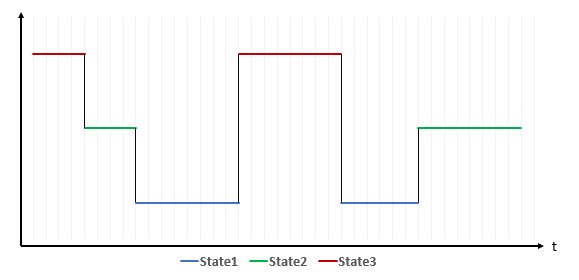
\includegraphics[width=0.5\linewidth]{graph3}
\end{figure}

\end{frame}


%------------------------------------------------
\begin{frame}
\frametitle{Markov switching model}
Assuming that $S_{t}$ denote an unobservable state variable

$$y_{t} = {X_{t}}'\beta_{S_{t}} + \varepsilon_{t}, \quad \varepsilon_{t} \sim N(0,\sigma^{2}_{S_{t}})$$

$y_{t}$ is the observed value of time series at time $t$ 

$X_{t}$ are the predictor variables of time series at time $t$ 

$\beta_{S_{t}}$ are the coefficients in state $S_{t}$, where $S_{t}=1,2,...,k$


\begin{figure}
	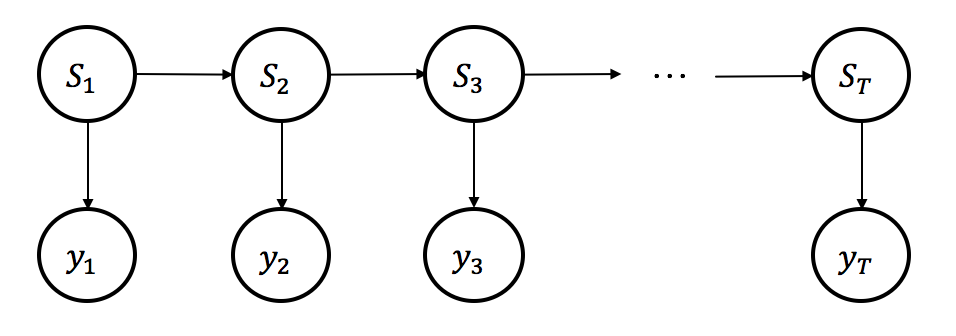
\includegraphics[width=0.5\linewidth]{msm}
	\caption{Model structure}
\end{figure}

\end{frame}

%------------------------------------------------

\begin{frame}
\frametitle{Markov switching model}

Given dataset,

\begin{itemize}
	\item $y_{t}$ is \textit{CPU utilization}
	\item$X_{t}$ are some components from the \textit{EventsPerSec} which have an impact on the \textit{CPU utilization} (e.g., \textit{RrcConnectionSetupComplete, Paging, X2HandoverRequest}) and test environment
	\item Assume there are three states ($k=3$): normal, good, bad
\end{itemize}

\begin{figure}
	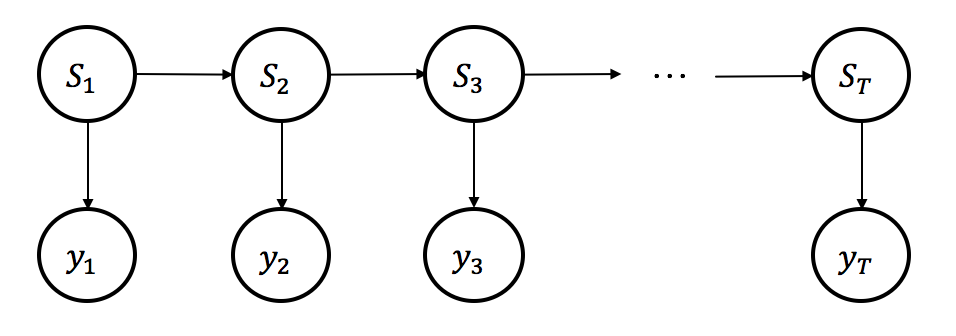
\includegraphics[width=0.5\linewidth]{msm}
	\caption{Model structure}
\end{figure}

\end{frame}

%------------------------------------------------
\subsection{Markov autoregression switching model} % A subsection can be created just before a set of slides with a common theme to further break down your presentation into chunks

\begin{frame}
\frametitle{Markov autoregression switching model}
The observation are drawn from the first order autoregressive model, AR(1), that is it depends on the past observation and the current state.

$$y_{t} = {X_{t}}' \beta_{S_{t}} + \phi_{1,S_{t}} y_{t-1} + \varepsilon_{t}$$

\begin{figure}
	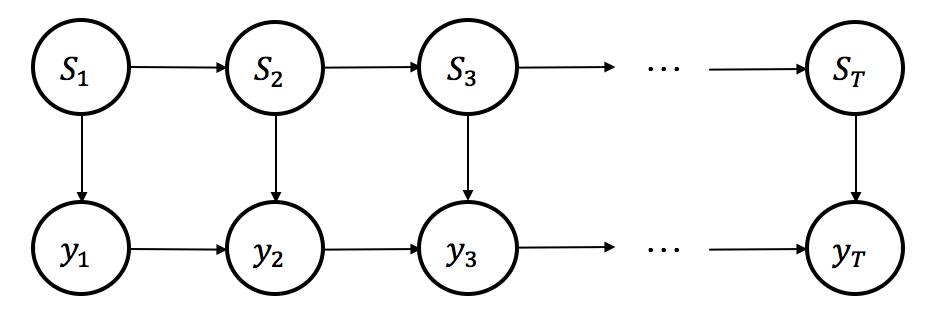
\includegraphics[width=0.5\linewidth]{msm-ar}
	\caption{Model with additional dependencies at observation level}
\end{figure}
\end{frame}

%------------------------------------------------
\section{What has been done?}
\begin{frame}
\frametitle{What has been done?}
\begin{itemize}
	\item Study and review source code  in the R package in detail
	\begin{itemize}
		\item MSwM: An univariate autoregressive Markov switching models for linear and generalized models
	\end{itemize}
	
	\item Implement and modify algorithm to fit with the problem and given dataset
	\begin{itemize}
		\item Categorical variables
		\item NAs coefficients
	\end{itemize}
	
	\item Solve computational problems
	\begin{itemize}
		\item Invertible Hessian
	\end{itemize}
\end{itemize}
\end{frame}

%------------------------------------------------
\section{Next step}
\begin{frame}
\frametitle{Next step}
\begin{itemize}
	\item Model Selection
	\begin{itemize}
		\item Compare several models (e.g., number of states, parameter which has switching effect)
		\item Select the most suitable model for a given set of data based on the quality of model (e.g., AIC, BIC)
	\end{itemize}
	\item State Prediction
	\begin{itemize}
		\item Training model using the set of parameters from the model in previous step
		\item Find the most probable state for the new observation
	\end{itemize}
	\item State Inference

\end{itemize}
\end{frame}


\end{document} 